
\documentclass[a4paper,11pt]{article}
\usepackage[a4paper, margin=8em]{geometry}

% usa i pacchetti per la scrittura in italiano
\usepackage[french,italian]{babel}
\usepackage[T1]{fontenc}
\usepackage[utf8]{inputenc}
\frenchspacing 

% usa i pacchetti per la formattazione matematica
\usepackage{amsmath, amssymb, amsthm, amsfonts}

% usa altri pacchetti
\usepackage{gensymb}
\usepackage{hyperref}
\usepackage{standalone}

\usepackage{colortbl}

\usepackage{xstring}
\usepackage{karnaugh-map}

% imposta il titolo
\title{Specification and Simulation of Digital Systems notes}
\author{Luca Seggiani}
\date{2026}

% imposta lo stile
% usa helvetica
\usepackage[scaled]{helvet}
% usa palatino
\usepackage{palatino}
% usa un font monospazio guardabile
\usepackage{lmodern}

\renewcommand{\rmdefault}{ppl}
\renewcommand{\sfdefault}{phv}
\renewcommand{\ttdefault}{lmtt}

% circuiti
\usepackage{circuitikz}
\usetikzlibrary{babel}

% testo cerchiato
\newcommand*\circled[1]{\tikz[baseline=(char.base)]{
            \node[shape=circle,draw,inner sep=2pt] (char) {#1};}}

% disponi il titolo
\makeatletter
\renewcommand{\maketitle} {
	\begin{center} 
		\begin{minipage}[t]{.8\textwidth}
			\textsf{\huge\bfseries \@title} 
		\end{minipage}%
		\begin{minipage}[t]{.2\textwidth}
			\raggedleft \vspace{-1.65em}
			\textsf{\small \@author} \vfill
			\textsf{\small \@date}
		\end{minipage}
		\par
	\end{center}

	\thispagestyle{empty}
	\pagestyle{fancy}
}
\makeatother

% disponi teoremi
\usepackage{tcolorbox}
\newtcolorbox[auto counter, number within=section]{theorem}[2][]{%
	colback=blue!10, 
	colframe=blue!40!black, 
	sharp corners=northwest,
	fonttitle=\sffamily\bfseries, 
	title=Theorem~\thetcbcounter: #2, 
	#1
}

% disponi definizioni
\newtcolorbox[auto counter, number within=section]{definition}[2][]{%
	colback=red!10,
	colframe=red!40!black,
	sharp corners=northwest,
	fonttitle=\sffamily\bfseries,
	title=Definition~\thetcbcounter: #2,
	#1
}

% disponi codice
\usepackage{listings}
\usepackage[table]{xcolor}

\definecolor{codegreen}{rgb}{0,0.6,0}
\definecolor{codegray}{rgb}{0.5,0.5,0.5}
\definecolor{codepurple}{rgb}{0.58,0,0.82}
\definecolor{backcolour}{rgb}{0.95,0.95,0.92}

\lstdefinestyle{codestyle}{
		backgroundcolor=\color{black!5}, 
		commentstyle=\color{codegreen},
		keywordstyle=\bfseries\color{magenta},
		numberstyle=\sffamily\tiny\color{black!60},
		stringstyle=\color{green!50!black},
		basicstyle=\ttfamily\footnotesize,
		breakatwhitespace=false,         
		breaklines=true,                 
		captionpos=b,                    
		keepspaces=true,                 
		numbers=left,                    
		numbersep=5pt,                  
		showspaces=false,                
		showstringspaces=false,
		showtabs=false,                  
		tabsize=2
}

\lstdefinestyle{shellstyle}{
		backgroundcolor=\color{black!5}, 
		basicstyle=\ttfamily\footnotesize\color{black}, 
		commentstyle=\color{black}, 
		keywordstyle=\color{black},
		numberstyle=\color{black!5},
		stringstyle=\color{black}, 
		showspaces=false,
		showstringspaces=false, 
		showtabs=false, 
		tabsize=2, 
		numbers=none, 
		breaklines=true
}

\lstdefinelanguage{x86}{ 
  keywords={AAA, AAD, AAM, AAS, ADC, ADCB, ADCW, ADCL, ADD, ADDB, ADDW, ADDL, AND, ANDB, ANDW, ANDL,
        ARPL, BOUND, BSF, BSFL, BSFW, BSR, BSRL, BSRW, BSWAP, BT, BTC, BTCB, BTCW, BTCL, BTR, 
        BTRB, BTRW, BTRL, BTS, BTSB, BTSW, BTSL, CALL, CBW, CDQ, CLC, CLD, CLI, CLTS, CMC, CMP,
        CMPB, CMPW, CMPL, CMPS, CMPSB, CMPSD, CMPSW, CMPXCHG, CMPXCHGB, CMPXCHGW, CMPXCHGL,
        CMPXCHG8B, CPUID, CWDE, DAA, DAS, DEC, DECB, DECW, DECL, DIV, DIVB, DIVW, DIVL, ENTER,
        HLT, IDIV, IDIVB, IDIVW, IDIVL, IMUL, IMULB, IMULW, IMULL, IN, INB, INW, INL, INC, INCB,
        INCW, INCL, INS, INSB, INSD, INSW, INT, INT3, INTO, INVD, INVLPG, IRET, IRETD, JA, JAE,
        JB, JBE, JC, JCXZ, JE, JECXZ, JG, JGE, JL, JLE, JMP, JNA, JNAE, JNB, JNBE, JNC, JNE, JNG,
        JNGE, JNL, JNLE, JNO, JNP, JNS, JNZ, JO, JP, JPE, JPO, JS, JZ, LAHF, LAR, LCALL, LDS,
        LEA, LEAVE, LES, LFS, LGDT, LGS, LIDT, LMSW, LOCK, LODSB, LODSD, LODSW, LOOP, LOOPE,
        LOOPNE, LSL, LSS, LTR, MOV, MOVB, MOVW, MOVL, MOVSB, MOVSD, MOVSW, MOVSX, MOVSXB,
        MOVSXW, MOVSXL, MOVZX, MOVZXB, MOVZXW, MOVZXL, MUL, MULB, MULW, MULL, NEG, NEGB, NEGW,
        NEGL, NOP, NOT, NOTB, NOTW, NOTL, OR, ORB, ORW, ORL, OUT, OUTB, OUTW, OUTL, OUTSB, OUTSD,
        OUTSW, POP, POPL, POPW, POPB, POPA, POPAD, POPF, POPFD, PUSH, PUSHL, PUSHW, PUSHB, PUSHA, 
        RCLL, RCR, RCRB, RCRW, RCRL, RDMSR, RDPMC, RDTSC, REP, REPE, REPNE, RET, ROL, ROLB, ROLW,
        ROLL, ROR, RORB, RORW, RORL, SAHF, SAL, SALB, SALW, SALL, SAR, SARB, SARW, SARL, SBB,
        SBBB, SBBW, SBBL, SCASB, SCASD, SCASW, SETA, SETAE, SETB, SETBE, SETC, SETE, SETG, SETGE,
        SETL, SETLE, SETNA, SETNAE, SETNB, SETNBE, SETNC, SETNE, SETNG, SETNGE, SETNL, SETNLE,
        SETNO, SETNP, SETNS, SETNZ, SETO, SETP, SETPE, SETPO, SETS, SETZ, SGDT, SHL, SHLB, SHLW,
        SHLL, SHLD, SHR, SHRB, SHRW, SHRL, SHRD, SIDT, SLDT, SMSW, STC, STD, STI, STOSB, STOSD,
        STOSW, STR, SUB, SUBB, SUBW, SUBL, TEST, TESTB, TESTW, TESTL, VERR, VERW, WAIT, WBINVD,
        XADD, XADDB, XADDW, XADDL, XCHG, XCHGB, XCHGW, XCHGL, XLAT, XLATB, XOR, XORB, XORW, XORL},
  keywordstyle=\color{blue}\bfseries,
  ndkeywordstyle=\color{darkgray}\bfseries,
  identifierstyle=\color{black},
  sensitive=false,
  comment=[l]{\#},
  morecomment=[s]{/*}{*/},
  commentstyle=\color{purple}\ttfamily,
  stringstyle=\color{red}\ttfamily,
  morestring=[b]',
  morestring=[b]"
}

\lstdefinelanguage{riscv}{
  keywords={
    LUI, AUIPC,
    JAL, JALR,
    BEQ, BNE, BLT, BGE, BLTU, BGEU,
    LB, LH, LW, LBU, LHU, LD,
    SB, SH, SW, SD,
    ADDI, SLTI, SLTIU, XORI, ORI, ANDI,
    SLLI, SRLI, SRAI,
    ADD, SUB, SLL, SLT, SLTU, XOR, SRL, SRA, OR, AND,
    ADDIW, SLLIW, SRLIW, SRAIW,
    ADDW, SUBW, SLLW, SRLW, SRAW,
    MUL, MULH, MULHSU, MULHU, DIV, DIVU, REM, REMU,
    MULW, DIVW, DIVUW, REMW, REMUW,
    LR.W, SC.W, AMOSWAP.W, AMOADD.W, AMOXOR.W,
    AMOAND.W, AMOOR.W, AMOMIN.W, AMOMAX.W,
    AMOMINU.W, AMOMAXU.W,
    LR.D, SC.D, AMOSWAP.D, AMOADD.D, AMOXOR.D,
    AMOAND.D, AMOOR.D, AMOMIN.D, AMOMAX.D,
    AMOMINU.D, AMOMAXU.D,
    FLW, FSW,
    FMADD.S, FMSUB.S, FNMSUB.S, FNMADD.S,
    FADD.S, FSUB.S, FMUL.S, FDIV.S, FSQRT.S,
    FSGNJ.S, FSGNJN.S, FSGNJX.S,
    FMIN.S, FMAX.S,
    FCVT.W.S, FCVT.WU.S, FCVT.S.W, FCVT.S.WU,
    FMV.X.W, FMV.W.X,
    FEQ.S, FLT.S, FLE.S,
    FLD, FSD,
    FMADD.D, FMSUB.D, FNMSUB.D, FNMADD.D,
    FADD.D, FSUB.D, FMUL.D, FDIV.D, FSQRT.D,
    FSGNJ.D, FSGNJN.D, FSGNJX.D,
    FMIN.D, FMAX.D,
    FCVT.W.D, FCVT.WU.D, FCVT.D.W, FCVT.D.WU,
    FCVT.S.D, FCVT.D.S,
    FMV.X.D, FMV.D.X,
    FEQ.D, FLT.D, FLE.D,
    CSRRW, CSRRS, CSRRC,
    CSRRWI, CSRRSI, CSRRCI,
    FENCE.I,
    FENCE,
    ECALL, EBREAK,
    MRET, SRET, URET,
    WFI,
    SFENCE.VMA,
    NOP, LI, LA, MV,
    NOT, NEG, NEGW,
    SEQZ, SNEZ, SLTZ, SGTZ,
    BEQZ, BNEZ, BLEZ, BGEZ, BLTZ, BGTZ,
    BGT, BLE, BGTU, BLEU,
    J, JR, RET,
    CALL, TAIL,
    RDINSTRET, RDCYCLE, RDTIME,
    CSRR, CSRW, CSRS, CSRC,
    CSRWI, CSRSI, CSRCI
  },
  keywordstyle=\color{blue}\bfseries,
  ndkeywordstyle=\color{darkgray}\bfseries,
  identifierstyle=\color{black},
  sensitive=false,
  comment=[l]{\#},
  morecomment=[s]{/*}{*/},
  commentstyle=\color{purple}\ttfamily,
  stringstyle=\color{red}\ttfamily,
  morestring=[b]',
  morestring=[b]"
}

\lstdefinelanguage{arm}{
  keywords={
    ADC, ADD, AND, BIC, CMN, CMP, EOR, MOV, MVN,
    RSB, RSC, SBC, SUB, TST, TEQ,
    MLA, MLS, MUL, SMLAL, SMULL, UMLAL, UMULL,
    QADD, QSUB, QDADD, QDSUB,
    QADD16, QADD8, QASX, QSAX,
    QSUB16, QSUB8, QSAX, QSUBADDX,
    ASR, LSL, LSR, ROR, RRX,
    B, BL, BX, BLX,
    BXJ,
    BEQ, BNE, BCS, BHS, BCC, BLO,
    BMI, BPL, BVS, BVC,
    BHI, BLS, BGE, BLT, BGT, BLE,
    BAL,
    LDR, LDRB, LDRH, LDRSB, LDRSH,
    LDRD, LDM, LDMIA, LDMIB, LDMDA, LDMDB,
    LDRT, LDRBT, LDRHT, LDRSBT, LDRSHT,
    STR, STRB, STRH, STRD,
    STM, STMIA, STMIB, STMDA, STMDB,
    STRT, STRBT, STRHT,
    PUSH, POP,
    SWP, SWPB,
    REV, REV16, REVSH,
    BFC, BFI, BFXIL, SBFX, UBFX,
    CLZ,
    LDREX, LDREXB, LDREXH, LDREXD,
    STREX, STREXB, STREXH, STREXD,
    DMB, DSB, ISB,
    MCR, MCRR, MRC, MRRC,
    MRS, MSR,
    CPS, SETEND, SVC, BKPT,
    CLREX, WFE, WFI, SEV,
    YIELD, NOP,
    VLDR, VSTR,
    VMOV, VABS, VNEG,
    VADD, VSUB, VMUL, VDIV,
    VMLA, VMLS, VNMLA, VNMLS, VNMUL,
    VMAX, VMIN,
    VSQRT,
    VCMP, VCMPE,
    VCVT,
    VCLZ, VCLS,
    VAND, VORR, VEOR, VBIC, VMVN,
    VLD1, VLD2, VLD3, VLD4,
    VST1, VST2, VST3, VST4,
    ADR, ADCS, ADDS, SUBS, MOVS, ANDS, ORRS, EORS
  },
  keywordstyle=\color{blue}\bfseries,
  ndkeywordstyle=\color{darkgray}\bfseries,
  identifierstyle=\color{black},
  sensitive=false,
  comment=[l]{@},
  morecomment=[l]{;},
  morecomment=[s]{/*}{*/},
  commentstyle=\color{purple}\ttfamily,
  stringstyle=\color{red}\ttfamily,
  morestring=[b]',
  morestring=[b]"
}

\lstset{style=codestyle, language=C}

% disponi sezioni
\usepackage{titlesec}

\titleformat{\section}
	{\sffamily\Large\bfseries} 
	{\thesection}{1em}{} 
\titleformat{\subsection}
	{\sffamily\large\bfseries}   
	{\thesubsection}{1em}{} 
\titleformat{\subsubsection}
	{\sffamily\normalsize\bfseries} 
	{\thesubsubsection}{1em}{}

% tikz
\usepackage{tikz}

% float
\usepackage{float}

% grafici
\usepackage{pgfplots}
\pgfplotsset{width=10cm,compat=1.9}

% disponi alberi
\usepackage{forest}

\forestset{
	rectstyle/.style={
		for tree={rectangle,draw,font=\large\sffamily}
	},
	roundstyle/.style={
		for tree={circle,draw,font=\large}
	}
}

% disponi algoritmi
\usepackage{algorithm}
\usepackage{algorithmic}
\makeatletter
\renewcommand{\ALG@name}{Algorithm}
\makeatother

% disponi numeri di pagina
\usepackage{fancyhdr}
\fancyhf{} 
\fancyfoot[L]{\sffamily{\thepage}}

\makeatletter
\fancyhead[L]{\raisebox{1ex}[0pt][0pt]{\sffamily{\@title \ \@date}}} 
\fancyhead[R]{\raisebox{1ex}[0pt][0pt]{\sffamily{\@author}}}
\makeatother

\begin{document}
% sezione (data)
\section{Lesson 02-10-26}

% stili pagina
\thispagestyle{empty}
\pagestyle{fancy}

% testo
In the last lesson we introduced \textit{combinatorial} circuits.

\subsection{Datapath components}

We now move on to increasingly complex digital building blocks:
\begin{itemize}
	\item \textbf{Combinational}: gates, multiplexors, decoders, ...;
	\item \textbf{Sequential}: basic registers, Finite State Machines, controller;
\end{itemize}

There is a notion of \textit{control}: \textit{controllers} are good for systems with control inputs/outputs, as opposed to data:
\begin{itemize}
	\item \textbf{Control input}: single bit (or a few), representing environment event or state;
	\item \textbf{Data input}: multiple bits representing single entity.
\end{itemize}

Our focus will be on \textbf{datapath} components at the register-transfer-level, or \textbf{RTL}.
These are usually networks \textit{controlled} by control networks, which perform functions with both:
\begin{itemize}
	\item Components to \textbf{store} data: registers;
	\item Components to \textbf{transform} data: functional blocks.
\end{itemize}

\subsubsection{Multiplexers}

We know from theory that \textbf{multiplexers} can implement any combinational logic function (basically a variation on \textit{Shannon's theorem}).
This means that they can serve as \textbf{LUT}s (\textit{Look Up Tables}) in FPGAs.

A few approaches can be proposed:
\begin{enumerate}
	\item An $m \times 2^n$ to $1$ multiplexer can implement $m$ functions of $n$ inputs. The steps are:
\begin{itemize}
	\item Write the truth tables for the $m$ functions;
	\item Use the $n$ inputs as selection signals for the multiplexer;
	\item Label the $m$ multiplexer outputs with the output functions;
	\item Set to 0 or 1 according to each truth table the data inputs of the multiplexer
\end{itemize}
	\item An inverter and an $m \times 2^n$ to $1$ multiplexer can implement $m$ functions of $n$ inputs. The steps are:
		\begin{itemize}
\item Write the truth tables for the m functions
\item Based on $n-1$ inputs identify pairs of rows in the tables
\item For each pair and output, identify an elementary function of the $n$-th input $X$ (that is constant 0 or 1, or $X$ or its negation); 
\item Using the first $n-1$ inputs as indices, assign the data inputs of the multiplexer with the appropriate elementary functions.
		\end{itemize}
\end{enumerate}

The inverter is clearly used to generate $X'$ (negation) in the elementary function, if needed.

\subsubsection{Adders}

Let's now focus on \textbf{adders}.
Adders have the (apparently) trivial job of adding toghether two $N$ bit binary numbers.

\par\smallskip
\textbf{\textsf{Table approach}}

They can be designed using combinational design procedures, but this doesn’t work well for typical $N$ (8, 16, 32, ...).
The approach scales terribly, as the truth table simply becomes too big to be directly expressed via Shannon expansion.

\par\smallskip
\textbf{\textsf{Hierarchical approach}}

The idea, then, is to implement in hardware what we usually do to sum numbers by hand:
\begin{enumerate}
	\item One column at a time;
	\item Compute sum of single column;
	\item Carry to next column;
	\item Repeat until done.
\end{enumerate}

This is trivial (and boring) in hardware, with ripple carry:
\begin{center}
	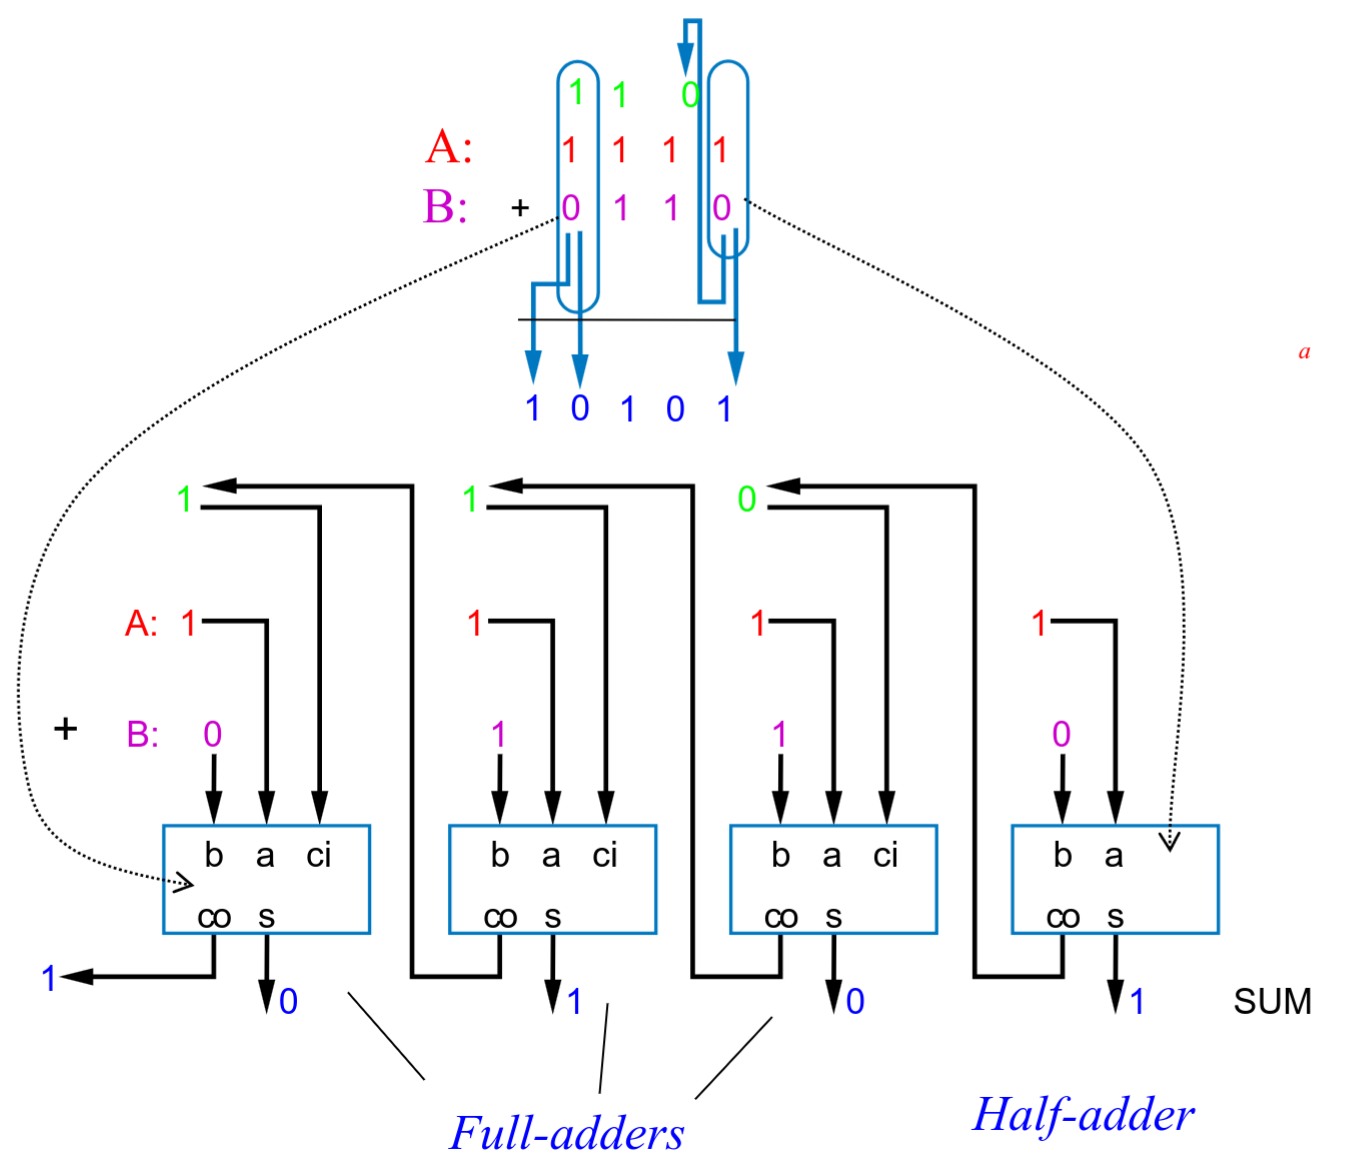
\includegraphics[scale=0.25]{../figures/adder.png}
\end{center}

Two components are used in the figure: an \textit{half adder}, and a set of \textit{adders}.
Using half-adder and full-adders, we can build adder that adds like
we would by hand:
\begin{itemize}
	\item The component is called a \textit{ripple-carry adder};
\item 4-bit adder shown: Adds two 4-bit numbers, generates 5-bit output;
\item 5-bit output can be considered 4-bit “sum” plus 1-bit “carry out”;
\item We can easily build any size adder.
\end{itemize}

\par\smallskip
\textbf{\textsf{Half adder}}

The \textbf{half adder} is the most trivial component: it takes 2 bits ($a$ and $b$) and returns:
\begin{itemize}
	\item $s$, the LSB of the sum of the bits;
	\item $c_{out}$, the MSB of the sum of the bits (they can evaluate to binary 2, which is 10).
\end{itemize}

The half adder is easy to implement both via LUTs, but also via discrete logic gates:
$$
s = a \otimes b, \quad c_{out} = a \cdot b
$$
where $\otimes$ is notation for XOR. 


\par\smallskip
\textbf{\textsf{Adder}}

The \textbf{adder} (or \textbf{full} \textit{adder}) is the slightly more complicated variant of the half adder: it sums 3 inputs instead of 2.
This is needed to correctly implement ripple carries, as we have the two digits at column $i$ plus the ripple carry from column $i - 1$ (which is always zero for the first digit, therefore justifying an half adder).

The full adder takes 3 bits ($a$, $b$ and $c_{in}$) and returns:
\begin{itemize}
	\item $s$, the LSB of the sum of the bits;
	\item $c_{out}$, the MSB of the sum of the bits (they can evaluate to binary 2, which is 10, or even binary 3, which is 11).
\end{itemize}

The full adder is easy to implement both via LUTs, but also via discrete logic gates or hierarchically, with half adders:
$$
s = a \otimes b \otimes c_{in}, \quad c_{out} = ab + ac_{in} + bc_{in} = (a \otimes b) \cdot c_{in} + a \cdot b
$$

Note that the XOR operator (again, $\otimes$) acts as a \textit{disparity checker} operator: for $\otimes_i^n \alpha_i$, if a odd number of $\alpha_i$ inputs are high, the XOR operator returns true. 

\par\smallskip

Note that using a full-adder instead of half-adder for first bit, we can include a “carry in” bit in the addition circuit.
This is useful later when we connect smaller adders to form bigger adders.

\par\smallskip
\textbf{\textsf{Adder timing characteristics}}

Ripple carry adders have specific timing behavoir: operations have to propagate (that is, \textit{ripple}) through all adder modules for the results to be correct.
This gives non-ideal timing characteristics (more bits mean significantly more delay, with linear scaling).

\subsubsection{Comparators}

We would now want to \textbf{compare} data, that is build a device which outputs 1 if two N-bit numbers are equal.

\par\smallskip
\textbf{\textsf{Equality comparator}}

If we are taking the \textbf{equality} of numbers, this is trivial. 
This is easy to achieve via XORs.
For instance, for 4 bits:
$$
eq = (a_3 b_3 + a_3' b_3') \cdot (a_2 b_2 + a_2' b_2') \cdot
     (a_1 b_1 + a_1' b_1') \cdot (a_0 b_0 + a_0' b_0')
$$

\begin{center}
	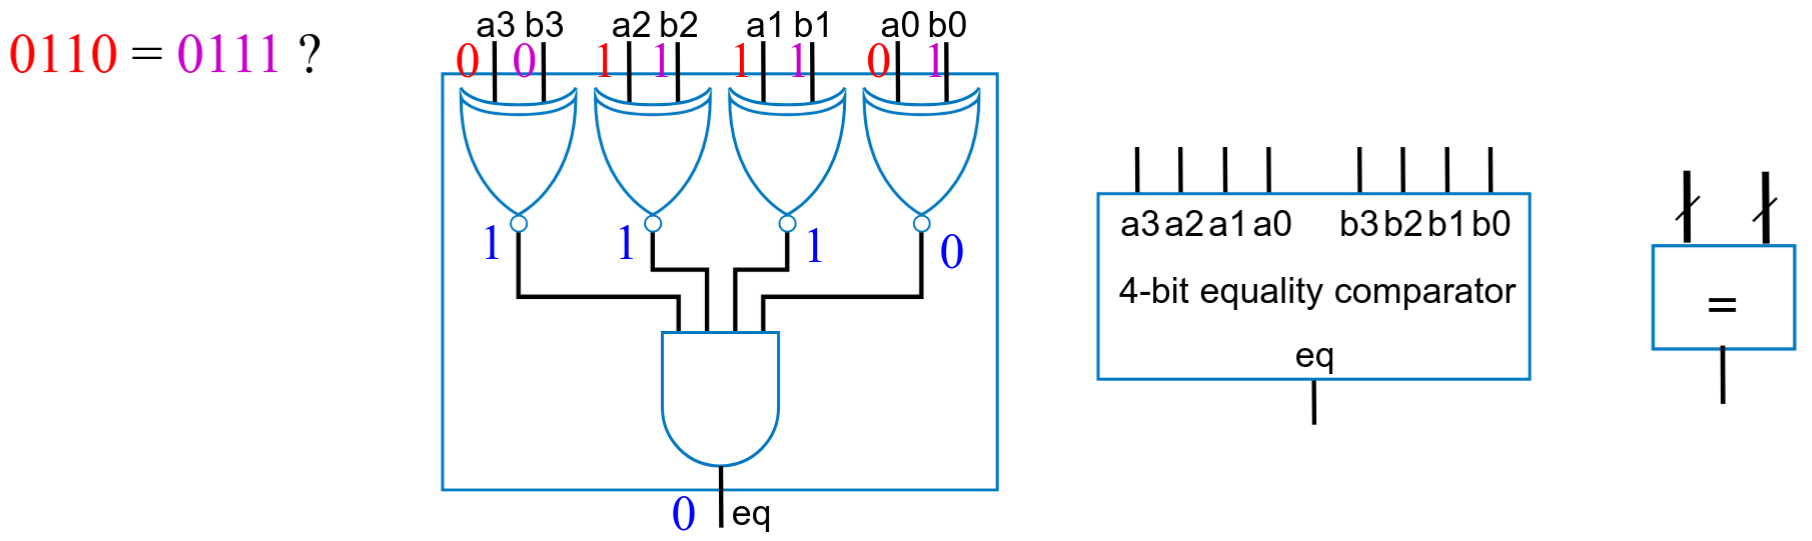
\includegraphics[scale=0.22]{../figures/comparator.png}
\end{center}

\par\smallskip
\textbf{\textsf{Magnitude comparator}}

We might also want a \textit{magnitude}, comparator.
We consider comparing by hand:
\begin{itemize}
\item First compare $a_3$ and $b_3$. If equal, compare $a_2$ and $b_2$. And so on;
\item Stop if comparison not equal (the two
bits are 0 and 1, or 1 and 0): 
whichever of A or B has the 1 is thus
greater.
\item If we never see an unequal bit pair,
then A=B.
\end{itemize}

This gives us the following circuit:
\begin{center}
	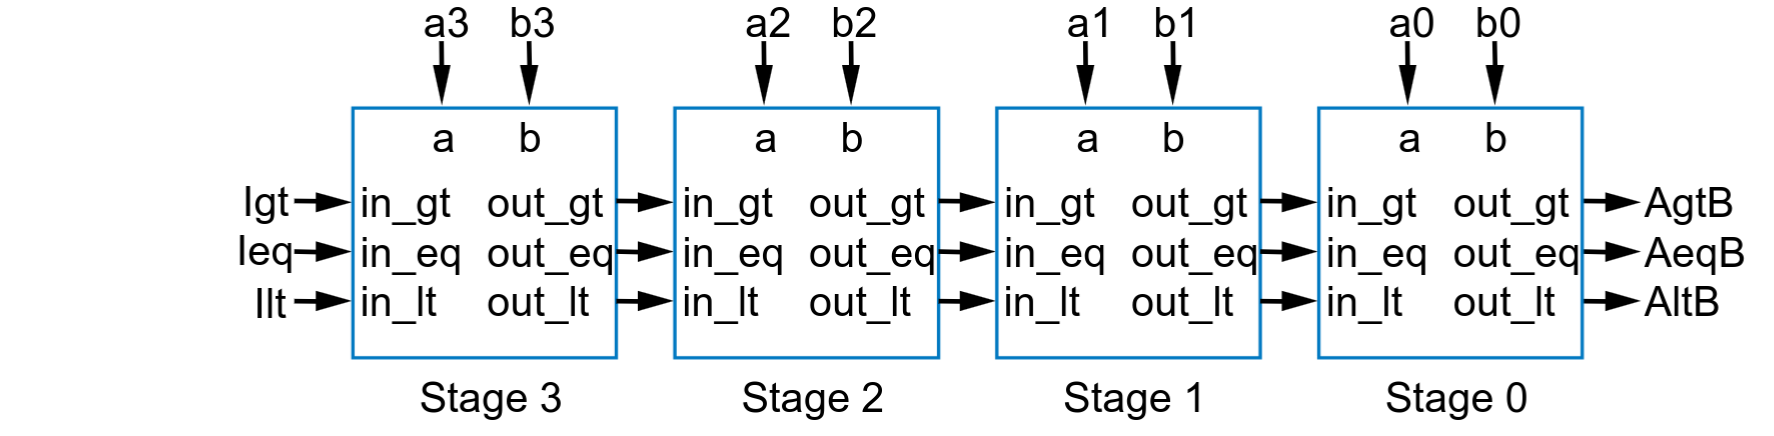
\includegraphics[scale=0.22]{../figures/mag_comparator.png}
\end{center}

Of course, we do need a single digit comparator.
Thankfully, this is easy to accomplish.

\subsubsection{Arithmetic Logic Units}

An \textbf{ALU} (\textit{Arithmetic Logic Unit}) is a component that can perform
various arithmetic (add, subtract,
increment, etc.) and logic (AND,
OR, etc.) operations, based on
control inputs.

\begin{center}
	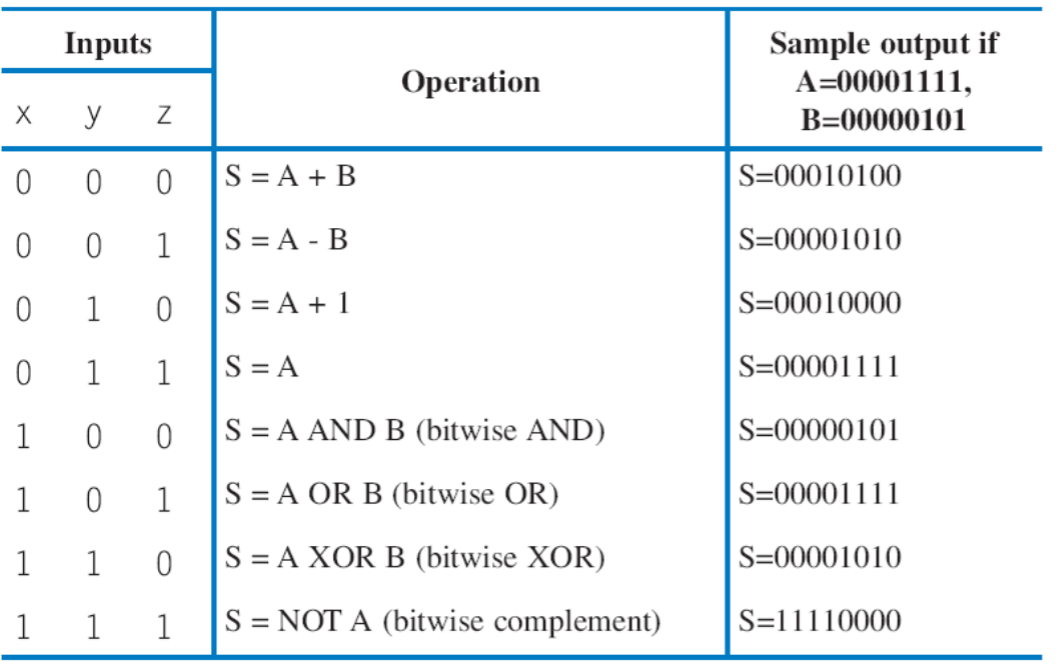
\includegraphics[scale=0.25]{../figures/alu.png}
\end{center}

\begin{itemize}
	\item 
The simplest way to implement an ALU is using separate
components for each operation, and
muxes. This, though, requires too many wires, and also wastes
power computing operations when we
only actually use one result at given time.
\item
Because of this, ALU designs don't just have separate components, multiplexed togheter.
Most ALU designs use a \textit{single adder}, plus logic in front of adder’s A and B inputs. 
This logic is called an \textbf{arithmetic-logic extender}: the extender modifies A and B inputs so desired operation appears at output of the adder
.

\begin{center}
	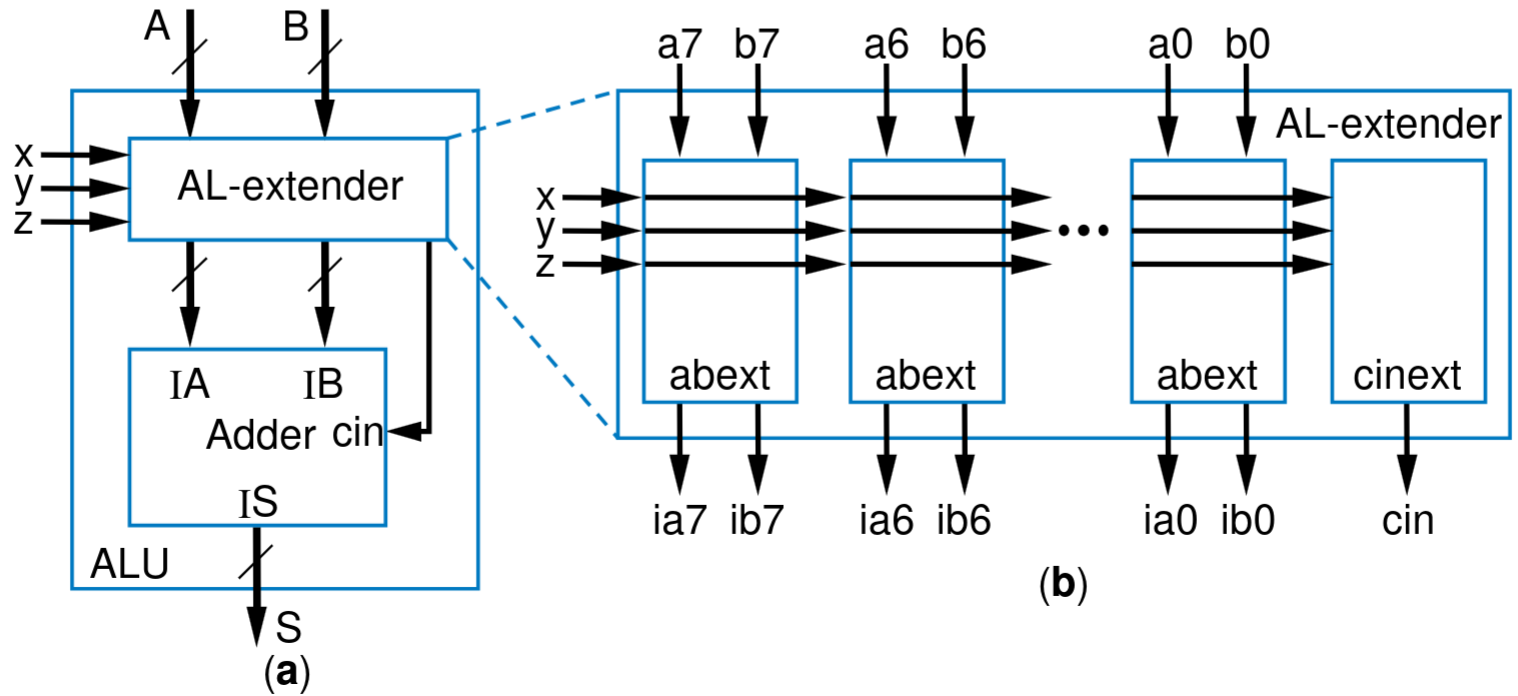
\includegraphics[scale=0.22]{../figures/extendo.png}
\end{center}

\end{itemize}

\subsection{VHDL delay models}

\lstset{language=VHDL}

There are 3 ways to model delays in VHDL:
\begin{enumerate}
	\item \textbf{Inertial delay} deletes pulses that are less than a threshold long. This is suitable for modeling delays through devise such as gate. The syntax is: \\ \lstinline|Y1 <= not(A and B) after 7ns;|

	\item \textbf{Transport delay} transports all pulses, i.e., all input events are propagated to output signals. It models delays through devices with very small inertia, e.g, wires: seldom used in hardware design. The syntax is: \\ \lstinline|Y2 <= not(A and B) transport after 7ns;|

	\item \textbf{Delta delay} means no propagation delays are specified.
Infinitesimally small delay is automatically inserted by the
simulator to preserve correct ordering of events (projected
values become current values).
\end{enumerate}

\end{document}
